\lecture{6}{mercredi 04 mars 2020}
\vspace{-1.2cm}

\section{Aspects morpho-lexicaux}

\epigraph{Language is mankind's greatest invention \\- except, of course, that it was never invented!}{\textit{G. Deutscher, 2005, in "The unfolding of language"}}

\textbf{Langages rationnels vs naturels}

La grammaire naturelle est composées de règles MAIS contient de nombreuses exceptions. Il est difficile (si pas impossible) d'anticiper toutes les évolutions de la langue:

\begin{enumerate}
    \item pluriels irréguliers
    \item néologismes
    \item langages SMS/tweets
    \item jargon technique
    \item ...\\
\end{enumerate}

\textbf{Abstraction}

Pour formaliser le langage naturel il est nécessaire de faire abstraction de nombreuses richesses. Ces simplifications sont nécessaires mais réductrices. Elles sont souvent limitées à un domaine précis et clos:

\begin{enumerate}
    \item météo
    \item réservations
    \item ELIZA
    \item ...\\
\end{enumerate}

\textbf{Exemples de langages rationnels}

Parler mouton: bê, bêê, bêêê, bêêêê

Rires: haha!, hihihi, hahahaha!

\subsection{Grammaires régulières}

Règles de réécriture: constituant $\rightarrow$ constitué

Majuscules = symboles; minuscules = littéraux

Règles récursives: même symbole utilisé à gauche et à droite de la flèche de réécriture\\

Exemple du parler mouton:

$ X \rightarrow bY $

$ Y \rightarrow \hat e Y $

$ Y \rightarrow \hat e $

\subsection{Expressions régulières (regex)}

Permettent d'exprimer des grammaires régulières de manière plus concise.

Sujet complexe et vaste, syntaxe ésotérique.\\

Exemples:

/bê+/ (parler mouton)

/h[ai](h[ai])+  !?/ (rires)

/\textbackslash b[A-Z0-9.\_\%+-]+@[A-Z0-9-.]+\textbackslash .[A-Z]\{2,\}\textbackslash b/ (détection d'adresse email)\\

Exercices online: \url{http://regex.sketchengine.co.uk/}

Solutions:

1 - p.t /
2 - ap.?t /
3 - af+g.?k /
4 - [a-z][.?!]['")]? +[A-Z]

\subsection{Automates finis}

FSA: Finite-State Automata (pluriel de Automaton)

Automate à nombre fini d'états (pas à états finis!)

Les transitions d'un état à un autre sont soumises à la satisfaction d'une condition.

\vspace{0.5cm}

\begin{center}
\resizebox{0.50\textwidth}{!}{
    \tikzset{every picture/.style={line width=0.75pt}} %set default line width to 0.75pt

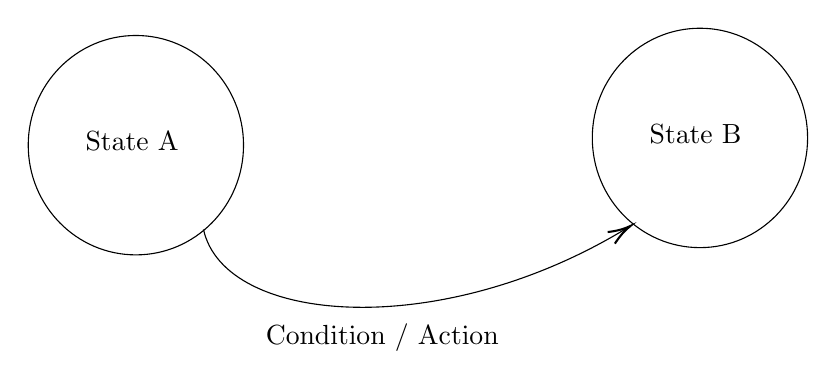
\begin{tikzpicture}[x=0.75pt,y=0.75pt,yscale=-1,xscale=1]
%uncomment if require: \path (0,777); %set diagram left start at 0, and has height of 777

%Shape: Ellipse [id:dp7032860404022366]
\draw   (10,63.35) .. controls (10,34.16) and (33.22,10.49) .. (61.87,10.49) .. controls (90.51,10.49) and (113.73,34.16) .. (113.73,63.35) .. controls (113.73,92.54) and (90.51,116.2) .. (61.87,116.2) .. controls (33.22,116.2) and (10,92.54) .. (10,63.35) -- cycle ;
%Shape: Ellipse [id:dp2228367254212833]
\draw   (281.77,59.85) .. controls (281.77,30.66) and (304.99,7) .. (333.63,7) .. controls (362.28,7) and (385.5,30.66) .. (385.5,59.85) .. controls (385.5,89.05) and (362.28,112.71) .. (333.63,112.71) .. controls (304.99,112.71) and (281.77,89.05) .. (281.77,59.85) -- cycle ;
%Curve Lines [id:da7146299088305332]
\draw    (94.44,103.97) .. controls (104.68,150.04) and (209.13,158.06) .. (298.85,103.06) ;
\draw [shift={(300.2,102.23)}, rotate = 508.15] [color={rgb, 255:red, 0; green, 0; blue, 0 }  ][line width=0.75]    (10.93,-3.29) .. controls (6.95,-1.4) and (3.31,-0.3) .. (0,0) .. controls (3.31,0.3) and (6.95,1.4) .. (10.93,3.29)   ;

% Text Node
\draw (36.37,55.72) node [anchor=north west][inner sep=0.75pt]   [align=left] {State A};
% Text Node
\draw (308.13,52.23) node [anchor=north west][inner sep=0.75pt]   [align=left] {State B};
% Text Node
\draw (123.18,148.33) node [anchor=north west][inner sep=0.75pt]   [align=left] {Condition / Action};
\end{tikzpicture}

}
\end{center}

\vspace{0.5cm}

\begin{minipage}[t]{0.6\textwidth}
États: représentés par des cercles

- État initial (triangle/flèche isolée)

- États intermédiaires

- État final (double cercle)\\
\end{minipage}
\begin{minipage}[t]{0.8\textwidth}
Transitions: représentées par des flèches

- D'un état à un autre

- D'un état à lui-même (récursif)

- Transition lambda/epsilon (vide)\\
\end{minipage}

\begin{center}
\resizebox{0.6\textwidth}{!}{
    \tikzset{every picture/.style={line width=0.75pt}} %set default line width to 0.75pt

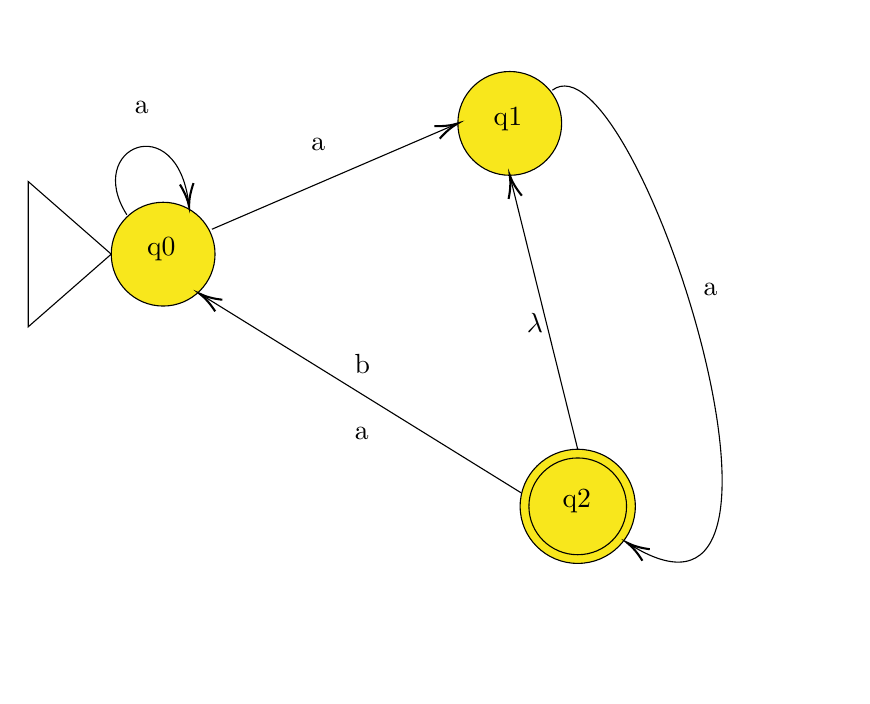
\begin{tikzpicture}[x=0.75pt,y=0.75pt,yscale=-1,xscale=1]
%uncomment if require: \path (0,777); %set diagram left start at 0, and has height of 777

%Flowchart: Extract [id:dp2213490168388459]
\draw   (48,96) -- (8,131) -- (8,61) -- cycle ;
%Shape: Circle [id:dp9156481012483882]
\draw  [fill={rgb, 255:red, 248; green, 231; blue, 28 }  ,fill opacity=1 ] (48,96) .. controls (48,82.19) and (59.19,71) .. (73,71) .. controls (86.81,71) and (98,82.19) .. (98,96) .. controls (98,109.81) and (86.81,121) .. (73,121) .. controls (59.19,121) and (48,109.81) .. (48,96) -- cycle ;
%Shape: Circle [id:dp8937236461295127]
\draw  [fill={rgb, 255:red, 248; green, 231; blue, 28 }  ,fill opacity=1 ] (215,33) .. controls (215,19.19) and (226.19,8) .. (240,8) .. controls (253.81,8) and (265,19.19) .. (265,33) .. controls (265,46.81) and (253.81,58) .. (240,58) .. controls (226.19,58) and (215,46.81) .. (215,33) -- cycle ;
%Shape: Ellipse [id:dp6295802993903136]
\draw  [fill={rgb, 255:red, 248; green, 231; blue, 28 }  ,fill opacity=1 ] (245,217.5) .. controls (245,202.31) and (257.42,190) .. (272.75,190) .. controls (288.08,190) and (300.5,202.31) .. (300.5,217.5) .. controls (300.5,232.69) and (288.08,245) .. (272.75,245) .. controls (257.42,245) and (245,232.69) .. (245,217.5) -- cycle ;
%Shape: Ellipse [id:dp23912526643664667]
\draw  [fill={rgb, 255:red, 248; green, 231; blue, 28 }  ,fill opacity=1 ] (249.23,217.5) .. controls (249.23,204.63) and (259.76,194.19) .. (272.75,194.19) .. controls (285.74,194.19) and (296.27,204.63) .. (296.27,217.5) .. controls (296.27,230.37) and (285.74,240.81) .. (272.75,240.81) .. controls (259.76,240.81) and (249.23,230.37) .. (249.23,217.5) -- cycle ;
%Straight Lines [id:da07722341343778594]
\draw    (245.5,211) -- (92.2,116.05) ;
\draw [shift={(90.5,115)}, rotate = 391.77] [color={rgb, 255:red, 0; green, 0; blue, 0 }  ][line width=0.75]    (10.93,-3.29) .. controls (6.95,-1.4) and (3.31,-0.3) .. (0,0) .. controls (3.31,0.3) and (6.95,1.4) .. (10.93,3.29)   ;
%Straight Lines [id:da5881939013667715]
\draw    (96.5,84) -- (213.16,33.79) ;
\draw [shift={(215,33)}, rotate = 516.71] [color={rgb, 255:red, 0; green, 0; blue, 0 }  ][line width=0.75]    (10.93,-3.29) .. controls (6.95,-1.4) and (3.31,-0.3) .. (0,0) .. controls (3.31,0.3) and (6.95,1.4) .. (10.93,3.29)   ;
%Curve Lines [id:da24978032388245308]
\draw    (260.5,17) .. controls (300.3,-12.85) and (399.5,298.86) .. (298.04,235.98) ;
\draw [shift={(296.5,235)}, rotate = 392.78999999999996] [color={rgb, 255:red, 0; green, 0; blue, 0 }  ][line width=0.75]    (10.93,-3.29) .. controls (6.95,-1.4) and (3.31,-0.3) .. (0,0) .. controls (3.31,0.3) and (6.95,1.4) .. (10.93,3.29)   ;
%Straight Lines [id:da3348378214953378]
\draw    (272.75,190) -- (240.48,59.94) ;
\draw [shift={(240,58)}, rotate = 436.07] [color={rgb, 255:red, 0; green, 0; blue, 0 }  ][line width=0.75]    (10.93,-3.29) .. controls (6.95,-1.4) and (3.31,-0.3) .. (0,0) .. controls (3.31,0.3) and (6.95,1.4) .. (10.93,3.29)   ;
%Curve Lines [id:da1693586185231678]
\draw    (55.5,77) .. controls (34.71,44.33) and (79.59,25.38) .. (85.34,71.58) ;
\draw [shift={(85.5,73)}, rotate = 264.05] [color={rgb, 255:red, 0; green, 0; blue, 0 }  ][line width=0.75]    (10.93,-3.29) .. controls (6.95,-1.4) and (3.31,-0.3) .. (0,0) .. controls (3.31,0.3) and (6.95,1.4) .. (10.93,3.29)   ;

% Text Node
\draw (247,123) node [anchor=north west][inner sep=0.75pt]   [align=left] {$\lambda$};
% Text Node
\draw (64,87) node [anchor=north west][inner sep=0.75pt]   [align=left] {q0};
% Text Node
\draw (231,24) node [anchor=north west][inner sep=0.75pt]   [align=left] {q1};
% Text Node
\draw (264.19,208.07) node [anchor=north west][inner sep=0.75pt]   [align=left] {q2};
% Text Node
\draw (58,21) node [anchor=north west][inner sep=0.75pt]   [align=left] {a};
% Text Node
\draw (332,109) node [anchor=north west][inner sep=0.75pt]   [align=left] {a};
% Text Node
\draw (143,39) node [anchor=north west][inner sep=0.75pt]   [align=left] {a};
% Text Node
\draw (164,143) node [anchor=north west][inner sep=0.75pt]   [align=left] {b\\ \\a};
\end{tikzpicture}

}
\end{center}

\textbf{Déterministe vs non-déterministe}

Après avoir reconnu "abb", sommes-nous à l'état final ou bien toujours à l'état initial? Impossible à dire avec certitude.

\begin{center}
\resizebox{\textwidth}{!}{
    \tikzset{every picture/.style={line width=0.75pt}} %set default line width to 0.75pt

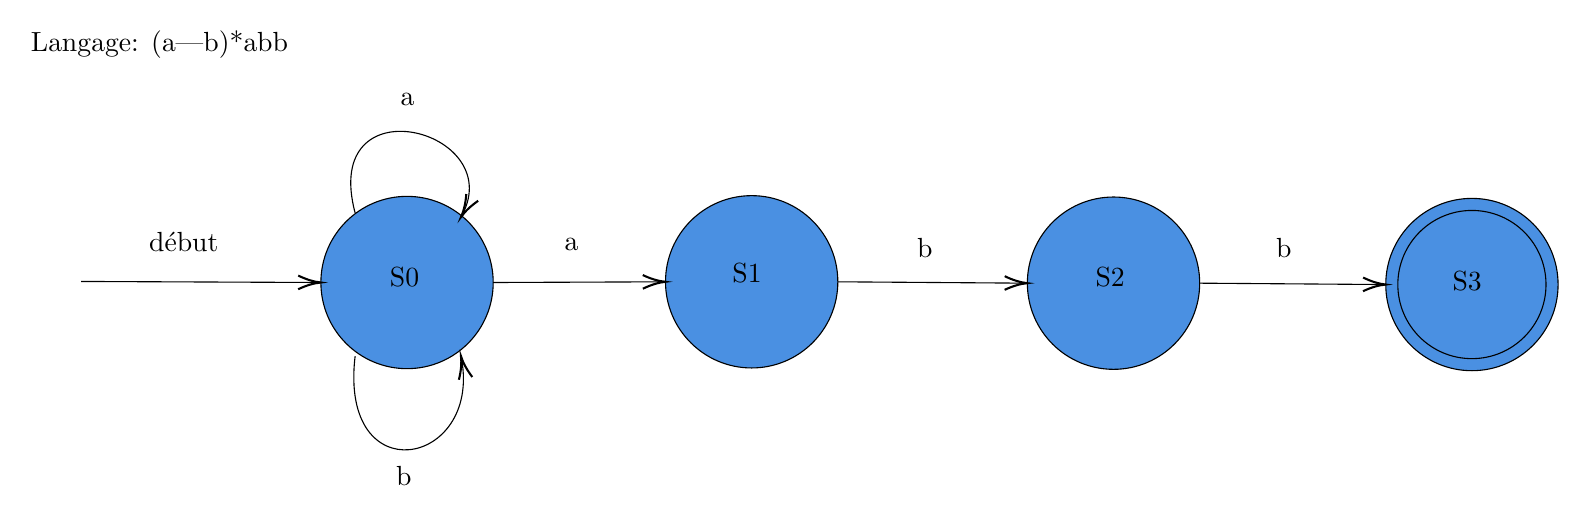
\begin{tikzpicture}[x=0.75pt,y=0.75pt,yscale=-1,xscale=1]
%uncomment if require: \path (0,777); %set diagram left start at 0, and has height of 777

%Shape: Circle [id:dp9851709242772706]
\draw  [fill={rgb, 255:red, 74; green, 144; blue, 226 }  ,fill opacity=1 ] (161,135.51) .. controls (161,112.58) and (179.58,94) .. (202.51,94) .. controls (225.43,94) and (244.02,112.58) .. (244.02,135.51) .. controls (244.02,158.43) and (225.43,177.02) .. (202.51,177.02) .. controls (179.58,177.02) and (161,158.43) .. (161,135.51) -- cycle ;
%Shape: Circle [id:dp2634550867663098]
\draw  [fill={rgb, 255:red, 74; green, 144; blue, 226 }  ,fill opacity=1 ] (327.04,135.17) .. controls (327.04,112.24) and (345.62,93.66) .. (368.55,93.66) .. controls (391.47,93.66) and (410.06,112.24) .. (410.06,135.17) .. controls (410.06,158.09) and (391.47,176.68) .. (368.55,176.68) .. controls (345.62,176.68) and (327.04,158.09) .. (327.04,135.17) -- cycle ;
%Shape: Circle [id:dp7244233597696788]
\draw  [fill={rgb, 255:red, 74; green, 144; blue, 226 }  ,fill opacity=1 ] (501.38,135.83) .. controls (501.38,112.91) and (519.96,94.32) .. (542.89,94.32) .. controls (565.81,94.32) and (584.4,112.91) .. (584.4,135.83) .. controls (584.4,158.76) and (565.81,177.34) .. (542.89,177.34) .. controls (519.96,177.34) and (501.38,158.76) .. (501.38,135.83) -- cycle ;
%Shape: Circle [id:dp07451760427696097]
\draw  [fill={rgb, 255:red, 74; green, 144; blue, 226 }  ,fill opacity=1 ] (674.06,136.49) .. controls (674.06,113.57) and (692.64,94.98) .. (715.57,94.98) .. controls (738.49,94.98) and (757.08,113.57) .. (757.08,136.49) .. controls (757.08,159.42) and (738.49,178) .. (715.57,178) .. controls (692.64,178) and (674.06,159.42) .. (674.06,136.49) -- cycle ;
%Shape: Ellipse [id:dp8941531755272224]
\draw  [fill={rgb, 255:red, 74; green, 144; blue, 226 }  ,fill opacity=1 ] (679.87,136.49) .. controls (679.87,116.78) and (695.85,100.79) .. (715.57,100.79) .. controls (735.28,100.79) and (751.26,116.78) .. (751.26,136.49) .. controls (751.26,156.21) and (735.28,172.19) .. (715.57,172.19) .. controls (695.85,172.19) and (679.87,156.21) .. (679.87,136.49) -- cycle ;
%Straight Lines [id:da9727164886338506]
\draw    (45.5,135) -- (159,135.5) ;
\draw [shift={(161,135.51)}, rotate = 180.25] [color={rgb, 255:red, 0; green, 0; blue, 0 }  ][line width=0.75]    (10.93,-3.29) .. controls (6.95,-1.4) and (3.31,-0.3) .. (0,0) .. controls (3.31,0.3) and (6.95,1.4) .. (10.93,3.29)   ;
%Straight Lines [id:da38657510871619216]
\draw    (244.02,135.51) -- (325.04,135.18) ;
\draw [shift={(327.04,135.17)}, rotate = 539.77] [color={rgb, 255:red, 0; green, 0; blue, 0 }  ][line width=0.75]    (10.93,-3.29) .. controls (6.95,-1.4) and (3.31,-0.3) .. (0,0) .. controls (3.31,0.3) and (6.95,1.4) .. (10.93,3.29)   ;
%Straight Lines [id:da45803946933994955]
\draw    (410.06,135.17) -- (499.38,135.82) ;
\draw [shift={(501.38,135.83)}, rotate = 180.41] [color={rgb, 255:red, 0; green, 0; blue, 0 }  ][line width=0.75]    (10.93,-3.29) .. controls (6.95,-1.4) and (3.31,-0.3) .. (0,0) .. controls (3.31,0.3) and (6.95,1.4) .. (10.93,3.29)   ;
%Straight Lines [id:da19707808507116387]
\draw    (584.4,135.83) -- (672.06,136.48) ;
\draw [shift={(674.06,136.49)}, rotate = 180.42] [color={rgb, 255:red, 0; green, 0; blue, 0 }  ][line width=0.75]    (10.93,-3.29) .. controls (6.95,-1.4) and (3.31,-0.3) .. (0,0) .. controls (3.31,0.3) and (6.95,1.4) .. (10.93,3.29)   ;
%Curve Lines [id:da7298553041692105]
\draw    (177.5,102) .. controls (160.67,38.64) and (250.67,61.53) .. (229.19,102.75) ;
\draw [shift={(228.5,104)}, rotate = 299.74] [color={rgb, 255:red, 0; green, 0; blue, 0 }  ][line width=0.75]    (10.93,-3.29) .. controls (6.95,-1.4) and (3.31,-0.3) .. (0,0) .. controls (3.31,0.3) and (6.95,1.4) .. (10.93,3.29)   ;
%Curve Lines [id:da9993413766624407]
\draw    (177.5,171) .. controls (169.58,237.33) and (238.11,224.27) .. (228.81,172.58) ;
\draw [shift={(228.5,171)}, rotate = 438.27] [color={rgb, 255:red, 0; green, 0; blue, 0 }  ][line width=0.75]    (10.93,-3.29) .. controls (6.95,-1.4) and (3.31,-0.3) .. (0,0) .. controls (3.31,0.3) and (6.95,1.4) .. (10.93,3.29)   ;

% Text Node
\draw (198,43) node [anchor=north west][inner sep=0.75pt]   [align=left] {a};
% Text Node
\draw (277,113) node [anchor=north west][inner sep=0.75pt]   [align=left] {a};
% Text Node
\draw (447,113) node [anchor=north west][inner sep=0.75pt]   [align=left] {b};
% Text Node
\draw (620,113) node [anchor=north west][inner sep=0.75pt]   [align=left] {b};
% Text Node
\draw (196,223) node [anchor=north west][inner sep=0.75pt]   [align=left] {b};
% Text Node
\draw (20,13) node [anchor=north west][inner sep=0.75pt]   [align=left] {Langage: (a|b)*abb};
% Text Node
\draw (77,110) node [anchor=north west][inner sep=0.75pt]   [align=left] {début};
% Text Node
\draw (193,127) node [anchor=north west][inner sep=0.75pt]   [align=left] {S0};
% Text Node
\draw (358,125) node [anchor=north west][inner sep=0.75pt]   [align=left] {S1};
% Text Node
\draw (533,127) node [anchor=north west][inner sep=0.75pt]   [align=left] {S2};
% Text Node
\draw (705,129) node [anchor=north west][inner sep=0.75pt]   [align=left] {S3};

\end{tikzpicture}

}
\end{center}

\newpage

\subsection{Équivalences}

On a décrit trois manières d'exprimer la même chose: les langages rationnels/réguliers/reconnaissables.

\begin{center}
\resizebox{0.6\textwidth}{!}{
    \tikzset{every picture/.style={line width=0.75pt}} %set default line width to 0.75pt

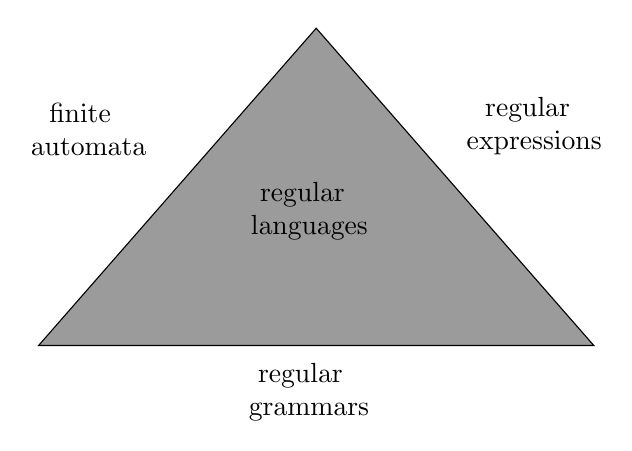
\begin{tikzpicture}[x=0.75pt,y=0.75pt,yscale=-1,xscale=1]
%uncomment if require: \path (0,777); %set diagram left start at 0, and has height of 777

%Shape: Triangle [id:dp3679553887605198]
\draw  [fill={rgb, 255:red, 155; green, 155; blue, 155 }  ,fill opacity=1 ] (152.75,10) -- (286.5,162.86) -- (19,162.86) -- cycle ;

% Text Node
\draw (120,83) node [anchor=north west][inner sep=0.75pt]   [align=left] { \ regular\\languages};
% Text Node
\draw (14,45) node [anchor=north west][inner sep=0.75pt]   [align=left] { \ \ finite\\automata};
% Text Node
\draw (224,42) node [anchor=north west][inner sep=0.75pt]   [align=left] { \ \ regular\\expressions};
% Text Node
\draw (119,170) node [anchor=north west][inner sep=0.75pt]   [align=left] { \ regular\\grammars};
\end{tikzpicture}

}
\end{center}

\subsection{Morphologie}

La morphologie permet soit de gérer des variantes de mots (morphologie flexionelle) soit de construire des nouveaux mots. \\

Au niveau de la construction, on peut soit faire une dérivation ("affixation", en conservant ou changeant la catégorie du mot) soit faire de la composition (noms composés, adjectifs composés, verbes composés, adverbes composés). \\

\subsection{Transducteurs}

FST: Finite-state transducers.\\

Similaires aux FSA mais la condition pour passer d'un état à un autre est remplacée par une action à effectuer. Utilisés soit pour analyser une chaine existante, soit pour générer une chaîne à partir de traits.\\

\subsection{Stemming}

\textbf{Racinisation (stemming)}

Version simplifiée de l'analyse morphologique. Ne s'encombre pas du lexique: principalement basée sur la désuffixation (vs lemmatisation). Moins précise mais beaucoup plus rapide. Très utilisée par les moteurs de recherche.\\

\textbf{Porter stemmer}

Crée par Martin Porter (1980). Ensemble de règles simples en cascade, par exemple:

\begin{itemize}
    \item SSES $\rightarrow$ SS
    \item ING $\rightarrow$ epsilon
    \item ATIONAL $\rightarrow$ ATE\\
\end{itemize}

Mais, ce n'est pas hyper précis, il y a de nombreux problèmes, comme par exemple:

\begin{itemize}
    \item organization $\rightarrow$ organ (sens perdu)
    \item policy $\rightarrow$ police (sens perdu)
    \item Adobe Illustrator $\rightarrow$ illustrate (nom propre a un sens particulier)\\
\end{itemize}

\subsection{Segmentation (tokenization)}

Séparation d'un texte en phrases et des phrases en mots. Étape cruciale pour le succès des stades suivants (analyse morphologique, traduction automatique, etc).\\

\textbf{Séparation en phrases}

Approche naïve: séparation par un point suivi d'un espace. Mais malheureusement cela ne couvre absolument pas tous les cas.\\

\textbf{Parts of Speech}

Les petites poules du couvent les couvent bien \\

\begin{minipage}[t]{0.5\textwidth}
\begin{itemize}
\item Les: DET
\item petites: ADJ
\item poules: NOM
\item du: PREP
\end{itemize}
\end{minipage}
\begin{minipage}[t]{0.5\textwidth}
\begin{itemize}
 \item couvent: NOM
\item les: PRON
\item couvent: VB
\item bien: ADV
\end{itemize}
\end{minipage}

\subsection{Tagging}

\textbf{Tagsets}

Listes des "parties du discours" (catégories)\\

Granularités très variables:
\begin{itemize}
    \item French Treebank: 15 catégories grammaticales
    \item Penn Treebank: 36 (45 avec la ponctuation)
    \item C5: 67
    \item Brown: 87
    \item Sinica (chinois): 294!\\
\end{itemize}

\textbf{PoS tagging}

Étiquetage morpho-syntaxique/grammatical.

Trois approches principales:
\begin{itemize}
    \item linguistiques (règles)
    \item statistique (HMM - hidden markov models, Viterbi)
    \item transformative (Brill tagger)\\
\end{itemize}

\textbf{Taggers linguistiques}

Choix parmi les différents candidats trouvés dans un dictionnaire. Basés sur une succession de règles très complexes. Exemple pour l'anglais: ENGTWOL.\\

\textbf{HMM taggers}

Approche probabiliste basée sur le modèle bayésien d'inférence (Hidden Markov Model - 1763). Choix de la séquence de tags la plus probable parmi toutes les séquences possibles, en fonction des mots observés.

Prémisses simplificatrices: la probabilité d'un mot ne dépend pas du contexte (faux, mais c'est pour simplifier); la probabilité d'un tag ne dépend que du précédent (modèle des bigrammes)

Approximation = produit entre: la probabilité d'un mot hors contexte (fréquence) pour un tag donné; la probabilité de transition d'un tag à un autre\\

\textbf{Brill tagger}

Approche hybride basée sur des règles ET un entrainement statistique (machine learning). Technique supervisée: nécessite un corpus annoté manuellement pour l'apprentissage. Première approximation probabiliste puis règles de transformation.
